\documentclass[12pt,a4paper]{article}
\usepackage[pdftex]{graphicx} %for embedding images
\usepackage{url} %for proper url entries
\usepackage[bookmarks, colorlinks=false, pdfborder={0 0 0}, pdftitle={<pdf title here>}, pdfauthor={<author's name here>}, pdfsubject={<subject here>}, pdfkeywords={<keywords here>}]{hyperref} 

\usepackage{lipsum}
\usepackage[margin=1in,includefoot]{geometry}
\usepackage{float}



\begin{document}
	%\renewcommand\bibname{References} 		%Renames "Bibliography" to 				"References"
	%\begin{titlepage}
\begin{center}
	\centering
	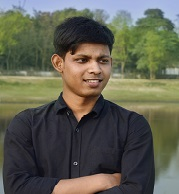
\includegraphics[width=0.15\textwidth]{/home/basedul/Documents/Report-writing-using-latex/ResturentManagementSystemReport/BasedulAppIcon.png}\par\vspace{1cm}
	{\scshape\LARGE Columbidae University \par}
	\vspace{1cm}
	{\scshape\Large Final year project\par}
	\vspace{1.5cm}
	{\huge\bfseries Pigeons love doves\par}
	\vspace{2cm}
	{\Large\itshape John Birdwatch\par}
	\vfill
	supervised by\par
	Dr.~Mark \textsc{Brown}

	\vfill

% Bottom of the page
	{\large \today\par}
\end{center}
\end{titlepage}
	
	\begin{titlepage}
	\begin{center}
	\centering
	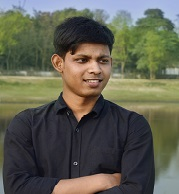
\includegraphics[width=0.15\textwidth]{/home/basedul/Documents/Report-writing-using-latex/ResturentManagementSystemReport/BasedulAppIcon.png}\par\vspace{1cm}
	{\scshape\LARGE Columbidae University \par}
	\vspace{1cm}
	{\scshape\Large Final year project\par}
	\vspace{1.5cm}
	{\huge\bfseries Pigeons love doves\par}
	\vspace{2cm}
	{\Large\itshape John Birdwatch\par}
	\vfill
	supervised by\par
	Dr.~Mark \textsc{Brown}

	\vfill

% Bottom of the page
	{\large \today\par}
\end{center}
\end{titlepage}
	
	\section*{ABSTRACT}
	This report documents the process of designing, developing and testing a software system to be used in a
restaurant; usually given the name restaurant management system. The restaurant management system
is there to help communication between all teams within a restaurant by minimising the probability
of human errors. This report was written by Carl Abernethy as part of his 3rd year project and was
published on May 5, 2010.\\
	\section*{ACKNOWLEDGEMENTS}
	I would like to thank my project supervisor, Prof. Chris Taylor, for providing an awful amount of
guidance and input throughout the writing of this report. In addition, I’d like to thank my family for
the support throughout my final year at university, and for checking over my report.\\

	\pagenumbering{roman} %numbering before main content starts
	
	\tableofcontents
	\newpage
	\listoffigures
	\listoftables
	
	\newpage
	\pagenumbering{arabic} %reset numbering to normal for the main content
	
	
	\section{INTODUCTION}
	The concept of restaurant table order management system, since it is java application, I will keep everything as simple as possible. The project consists in an java application that can be used by employees in a restaurant to handle the clients, their orders and can help them easily find free tables or place orders. This application, created mainly for proof of proper user-java interaction. The restaurant menu is organized by categories (appetizers, soups,fig salads, entrees, sides and dricks) of menu items. Each menu item has a chef, preparation instructions and associated in gredients. The ingredeints are identified by their ingredient id and the quality of the ingredient needed to prepare a particular recipe, the unit of measure and a name.
	\\
	"Restaurant Management System(RMS)" is java application to restaurant management. This system wake to provide service facility to retaurant and also to the customer. The services that are provided is food ordering and home delivery by the customer through the system, customer information management and waiter information management, menu information management and report. Main objective build the system, ordering, and home delivery management will become easier and systematic to replace traditional system.
	
	\subsection{EXISTING SYSTEM}
	\begin{itemize}
		\item Restaurant services such as making porcessing orders, and delivering meals generally require waiters to input customer information and then transmit the orders to kitchen for mela preparation. When the customer pays the bill, the amoutn due is calculated by the cashier. Although this procedure is simple, it may significantly increase the workload of waiters and even cause errors in meal ordering or in prioritizing customers, especially when the number o fcustomers suddenly increases during busy hours, which can seriusly degrade the overall service quality.
		\item A very commonly implemented system, currently being used by numerous restaurants and chains all over the world, is the electronic point-sale terminal system.
		\item Here the waiters generally take the order from the customer and head onto a terminal, where they can feed the order into a computer . The order can the be trasmitted to to the kitchen automatically via the terminal through the a network, or it may event be delivered manuallly by the server to the kitchen.
	\end{itemize}
	\subsubsection{DISADVANTAGES OF EXISTING SYSTEM}
	\begin{itemize}
		\item Although a huge improvement over the pen and paper still prevalent over world, this does not have much value addition for the customer and mostly only benegits the establilshment and the administration of the establishment.
		\item It may significantly increase the workload of waiters and even cause errors in meal ordering or in prioritizing customers, especially when the number of customers suddenly increases during busy hours, which can seriously dgrade the overall service quality.
	\end{itemize}
	
	
	\subsection{PROPOSED SYSTEM}
	\begin{itemize}
		\item The system will consist of the following main components: The backend, which is made up of the web server and the database, and the frontends tha include both the patro frontend and the administaration or the kitchen frontend 
		\item this system is based on the very popular model-View-Controller (MVC) architecture. MVC is most commonly used in websites, very popular and tried and tested. None of the frontends directly "talk" to the database. They instead rely on Restfull services that can be used to perform CRUD operations on the database.
	\end{itemize}
		
		\subsubsection{ADVANTAGES OF PROPOSED SYSTEM}
		\begin{itemize}
			\item The most important components of this system are the database and the frontends
			\item Providing value to both the business and its patron is an important objective, but we believe that one follows the other.
		\item Following that belief, the customer is given a whole lot of importance.
		\end{itemize}
		
	\subsection{MODULES}
		\begin{itemize}
			\item Customer
			\item Administrator
			\item Customer Ordering and home delevery
			\item Feedback Module
			\item Menu Module
			\item Generate Report Module
		\end{itemize}
		\subsubsection{MODULES DESCRIPTION}
		\begin{itemize}
			\item {\bfseries Customer} \\
			This project module consists in and java application tha can be used by employees in a restaurant to handle the cliens, their orders and can help them easily find free tables or place orders. This applicatio, created mainly for proof of proper user interacton.
			\item {\bfseries Administrator} \\
			Administrator is the person who will manage the entire system. This type of user will also do maintenance and control the application ot this system. Administrator thakes a responsibility to a new customer, new menu into database, and etc.
			\item {\bfseries Customer Ordering} \\
			Customer ordering and reservation module provides a from that needs to be fullfilling in term or ordering food.
			\item {\bfseries Menu Module } \\
			Menu module is food that restaurant prepared for customer. This module, customer can view the menu and make decision for order.
			\item {\bfseries Generate Report Module} \\
			System provides an option for generate a report. The contents of the report as following: \\
			1. The report of customer ordering. \\
			2. Customers information \\
			3. Comment or satisfiction score insert into feedback form.	
		\end{itemize}
		\subsection{Summary of Chapeters}
		The rest of this report consists of the following chapters: \\
		\begin{itemize}
			\item Background: Background investigation into the problem.
			\item Requirement Analysis: Requirements of the system including stakeholder identification, list of
features and tabulated requirements.
			\item Design: Project design process using several diagrammatic techniques.
			\item Implementation: Discusses the implementation of the software with the help of diagrams and
pseudocode.
			\item Results: Illustrates the system using screenshots.
			\item Testing: Documents how the system was tested.
			\item Conclusion: Project conclusion with future development ideas.
		\end{itemize}
	\subsection{Closing Remarks}
	This chapter has introduced the foundations of the project. The next chapter gives some background
investigation into the problem.

%%Second chapter

\newpage
\section{Chapter Two}
{\bfseries \Large Background} 
	\subsection{Chapter Overview}
	This chapter gives an insight to Point of Sale (POS) systems similar in nature to that of the one being
developed in this project. It also gives a brief introduction to the importance of requirement gathering,
a discussion on the development methodologies available as well as a justification on the platform and
software used in this project.
	\subsection{Point-of-Sale (POS) Systems}
	According to A. Nutt [12], POS systems first dated back to the 1870s, when James Ritty became
frustrated with dishonest employees stealing money from the customers in a saloon in Dayton, Ohio.
With the inspiration from a counter on a ship’s propeller that counted the number of revolutions, he
and his brother in 1879 developed the first cash register called ‘Ritty’s Incorruptible Cashier’.
By the 1970s, the first computerised cash register was developed that was basically a mainframe
but packaged as a store controller that had the ability to control the registers. Then in the 1980’s,
cash registers began to be PC operated which meant that many of the basic PC functions were now
available.
Today, the POS systems are much faster, safer and reliable and with the introduction of credit cards
and direct communication to the credit card company, transactions are almost instant.
\subsection{Platform Choice}
	Choosing a suitable platform normally goes down to the programmers experience and the type of
software to be developed. The restaurant management system could be developed as a web application
or a standalone application but must also be widely supported and platform-independent. Therefore
as the developer has minimal or no experience in web programming, the decision was taken to develop
a standalone application.
The next decision was to decide on a programming language, with the developer having previous
experience in C, C++ and Java. This decision was fairly easy and Java was the selected program-
ming language as the developer has great knowledge in the Java Database Connectivity (JDBC) API 1
that allows database-independent connectivity between the Java programming language and numerous
databases.
	\subsection{UML}
	\label{Sec:uml}
Diagrammatic techniques are used to visualise, construct and document software systems under de-
velopment. The most general modelling language to describe both the structure and behaviour of a
software system is Unified Modelling language (UML) created by the Object management group. The
diagrams one can create using UML can be shown by a class diagram (Figure \ref{fig:uml}). Throughout this
report, numerous models defined within the UML class diagram (Figure \ref{fig:uml}) will be used to graphically
represent the system.
	\begin{figure}
		\centering
		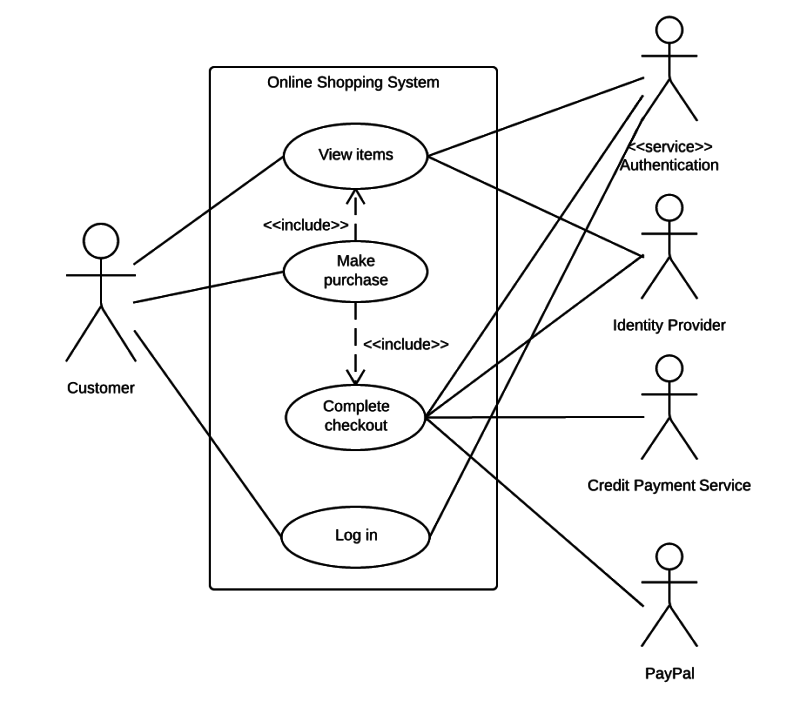
\includegraphics[height=2.5in]{/home/basedul/Documents/Report-writing-using-latex/ResturentManagementSystemReport/uml_case.PNG}
		\caption{UML diagram for Asian Restaurant Management system.}
		\label{fig:uml} 
	\end{figure}
	
	\subsection{Software Choice}
		In software development, the use of integrated development environments (IDE) can increase the effi-
ciency of a programmer. An IDE is a software application that consists of a source code editor, compiler
and debugging tools with its main aim to assist the programmer. Simple notepads are not strictly IDEs
but can do the same job with the assistance of a compiler.
The two most popular IDEs available for Java programming are Netbeans and Eclipse as they
are free, support multiple platforms and offer many features including integrated version control and
debugging tools. The two main problems with IDE’s are that due to the wealth of features available
and plug-in support, there is an associated cost, as their performance is poor and in particular they
require more memory and processing power than a standard text editor.
For this project Netbeans was the chosen IDE, as the developer has more experience and knowledge
of the Netbeans graphical user interface.
\subsection{Requirement Gathering}
	\begin{figure}
		\centering
		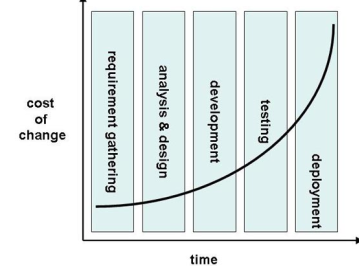
\includegraphics[height=5in]{/home/basedul/Documents/Report-writing-using-latex/ResturentManagementSystemReport/boehms.png}
		\caption{Boehm's cost model \cite{RefWorks:1}}
		\label{fig:req} 
	\end{figure}
	Requirement gathering is a very important step in software engineering. According to an article written
by Craig Murphy \cite{RefWorks:1}, Boehm’s cost model discusses how discovering errors at an early stage of software
development can reduce overall costs. Figure \ref{fig:req} is an example of Boehm’s cost model and uses the
waterfall technique to give a visual insight into how important gathering accurate requirements can be when the project has a strict deadline to work to. Roughly a £1 cost of change in the requirement
gathering can cost up to £100 in the testing stage and £1000 in the deployment stage to fix.
\newpage
\subsection{Development Methodology}
	A software development methodology is a framework used to plan the design of a software system
controlling the process of development. According to Geoffrey Elliott \cite{Ref:2}, software development meth-
odologies first emerged in the 1960’s with systems development life cycles (SDLC) being considered
the first formalised methodology. Since then there have been numerous popular software development
approaches including the waterfall model, prototyping, incremental, spiral and agile.
The agile methodology refers to a collection of different agile methods. This project will be based
on Extreme programming (XP) which is one of these agile methodologies using an iterative based
framework. Each iteration has a development cycle very similar to the waterfall model consisting
of planning, requirements analysis, design, development and testing. At each iteration, the business
representative sometimes referred to as the ‘customer’ is given a demonstration to promote useful
feedback. This type of methodology reduces risk and lets the project adapt to requested changes
quickly with minimum cost.\\
According to the Agile Manifesto \cite{Ref:3}, some of the main principles behind the agile methodology
are:
	\subsubsection{}
		\begin{itemize}
			\item Customer satisfaction by rapid, continuous delivery of useful software.
			\item Working software that is delivered frequently.
			\item A welcomed late change in requirements.
			\item Simplicity.
			\item Regular adaptation to changing circumstances.
		\end{itemize}

\subsection{Chapter Summary}
	
	This chapter has given examples of POS systems that are directly related to this project as well as
general information about requirement gathering and development methodologies. The next chapter
starts the process of the development methodology by generating the requirements of the system.
\newpage
\section{Chapter Three}
{\bfseries \Large Requirement Analysis}\\
\subsection{Chapter Overview}
	This chapter will look at the stakeholders of the system and then discuss the required features using a
use case diagram to illustrate.
\subsection{Stakeholder Identification}
	As defined in the Business Dictionary \cite{Ref:4},\\
a stakeholder could be a person, group, organisation that has direct or indirect stake in an
organization because it can affect or be affected by the organization’s actions, objectives
and policies.\\
Hence, stakeholders can be split into two groups; internal and external with each stakeholder contrib-
uting directly or indirectly towards the business activities.\\
As an example, any system were there exists customer communication, that customer will be a
non-financial beneficiary stakeholder.\\
According to an article written by Ian Alexander \cite{Ref:5}, the person,
group, organisation, or system is a stakeholder if they can be defined by any one of the following four
questions:\\

Who needs to be consulted on the scope of this project?\\

Who has an input to the budget of this project?\\

Who can support or harm this project politically?\\

Who can provide guidance on the usability, functionality, and required qualities (reliability,
safety, lifetime, maintainability, . . . ) of the system under development?\\

Therefore using these 4 questions as a guide, we can generate a list (\ref{tab:stake}) of the stakeholders
in this project.
\begin{table}[H]
	\centering
	\caption{A table showing the stakeholders of the project}
	\label{tab:stake}
	\begin{tabular}{l c r}
		\bfseries{Stakeholder} & \bfseries{Role}\\ \hline
		Carl Abernethy & Project developer.\\
		Prof. Chris Taylor & Project supervisor.\\
		Management & User of the management application.\\
		Waiters & User of the restaurant application.\\
		Kitchen Staff & User of the kitchen application.\\
		Bar Staff & User of the restaurant application.\\
		Customer & Indirect user of the system.\\
		Cashier & External stakeholder; accepts payment.\\
	\end{tabular}
\end{table}

\subsection{Use Cases}
	A use case diagram that is part of the Unified Modelling Language (UML) which was introduced in
Section \ref{Sec:uml} gives a graphical overview of the functionality of a system. A use case diagram consists of
actors that are normally the stakeholders of the system and their use cases commonly defined as goals.
Figure \ref{fig:usecase} shows several use case scenarios of the system that convey how the stakeholders interact
with the features to achieve a business requirement.
\begin{figure}[H]
		\centering
		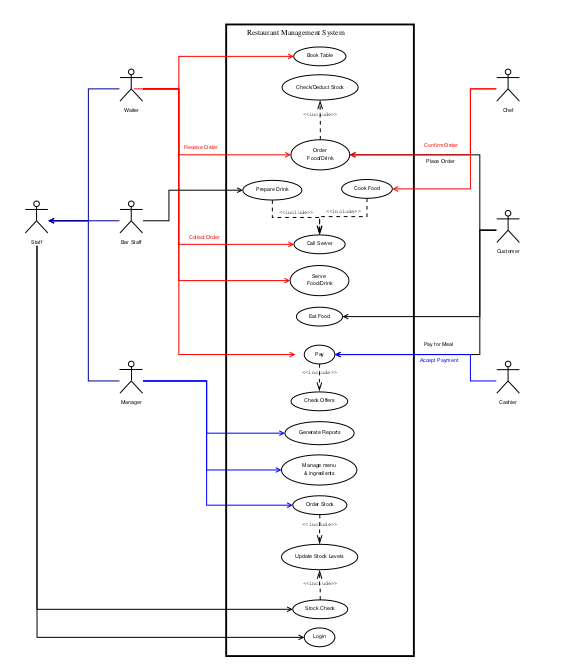
\includegraphics[height=7in]{/home/basedul/Documents/Report-writing-using-latex/ResturentManagementSystemReport/usecase.png}
		\caption{Use case diagram showing some of the major fearures with in the asian restaurant management system}
		\label{fig:usecase} 
	\end{figure}

The use case diagram is designed to be sequential so by following the use cases down the spine, one
can follow the major steps of an order and several post features to query the data.

\subsection{Features}
	An important part of requirements gathering is the production of a list of system features that cat-
egorises on priority.

	\begin{table}[H]
	\centering
	\caption{A table showing the proposed system features and allocated priorities.}
	\label{tab:fea}
	\begin{tabular}{l c r}
		\bfseries{Feature} & \bfseries{Priority}\\ \hline
		Communication of data between each application & 1\\
		Meal ingredient & 1\\ \hline
		Ability to define groups of ingredients that may be used in numerous meals & 2\\
		Flexible meal grid design to fit any screen size & 2\\ \hline
		User login functionality & 3\\
		Interface for table management and selection & 3\\
	\end{tabular}
\end{table}	
\subsection{Measureable Goals and Requirements}
	The measurable goals and requirements of the system are a list of manageable requirements and goals
for each application that can be prioritised and ‘ticked off’. The software requirements specification (SRS) is a complete list of requirements to be designed and developed and can take the form of functional
or non-functional requirements.
	
\subsection{Chapter Summary}
	This chapter has discussed the requirements of the system and the development methodology that will
be used throughout this project. The design of the system is documented in the next chapter.
\newpage
\section{Chapter Four}
{\bfseries\Large Design}
	\subsection{Chapter Overview}
	This chapter will focus on the design of the system using diagrams to illustrate graphically certain
sections of the software system.

	\subsection{Introduction}
	This project has been designed using numerous diagrammatic techniques. Recall from Section \ref{fig:uml}, that
the most general modelling language to describe both the structure and behaviour of a software system
is Unified Modelling language (UML).
Use case diagrams have already been used in the requirements analysis as a way to graphically
overview the order process within the system. Other diagrams from the UML family are used in the
design stage to show the structure and behaviour of numerous sophisticated design feature.
\subsection{Component Diagram}
A component diagram is part of UML and its main purpose is to show the structural relationship
between components in the system. A component diagram is useful for this system as it shows the
higher architecture, as shown in figure \ref{fig:comdia}
\begin{figure}[H]
		\centering
		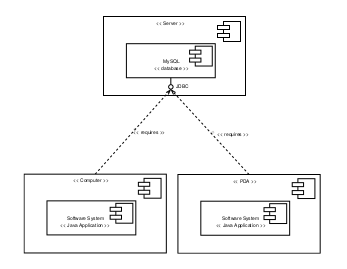
\includegraphics[height=3in]{/home/basedul/Documents/Report-writing-using-latex/ResturentManagementSystemReport/comdia.png}
		\caption{Component diagram showing the higher level architecture of the system.}
		\label{fig:comdia} 
	\end{figure}
	
\subsection{Data Storage}
	The restaurant management system will be built around the data storage technique therefore choosing
the most appropriate persistent 1 data storage is critical to a successful project and we can assume a flat
file storage approach is inadequate. The two most popular types of persistent data storage available
are relational database management system (RDBMS) and extensible markup language (XML)
\subsubsection{Relational Database Management System (RDBMS)}
	A relational database management system (RDBMS) is a database managed system based around a
relational model and are the corner stone’s to many software systems including web based systems.\\
RDBMS are one of the most popular data storage methods out in the market and offer many advantages
including:\\
\begin{itemize}
	\item Fast data extraction using structured query language (SQL).
	\item Good management of data and security through the management system.
	\item Good level of data consistency.
	\item Advanced features including functions and triggers.
	\item Requirement of a data model to be developed; leading to long term cost effectiveness. 
\end{itemize}
In industry, there are numerous expensive highly functional RDMBSs including Oracle and SQLServer
that are very popular and offer technical support. However, there are also numerous open-source solu-
tions with many adjudged to be as good or better and are becoming even more popular with small
scale software systems.
\subsubsection{Extensible Markup Language (XML)}
	XML is a markup language that was designed to transport and store data and is another example of
a persistent data storage technique. However, it is not a predefined language thus all tags must be
defined and due to its hierarchically data structure all elements must be promoted or demoted.
XML could be used in two different ways in data storage; storing the XML documents within a
database or having the XML documents as the fundamental unit of storage. In both cases the XML
can be queried using either XPATH or XQUERY which are query languages for extracting data from
XML documents.
\subsubsection{Storage Method Chosen}
	The main difference between XML and RDBMS is that XML is hierarchical and RDBMS is relational.
As restaurant data can be best represented in a hierarchical way one would believe that XML would be
the best approach but it’s not always that straight forward. SQL is an extremely flexible and robust querying language and for the queries required and the type of software system begin designed, it was
concluded that RDBMS would be the best storage method.
The next choice was to decide on the type of RDBMS to use. As discussed there are many open
source RDBMSs available for us to choose from and for the main reason of experience, MySQL was the
preferred option. Figure \ref{fig:compari} shows just how competitive the performances of different RDBMSs are.
\begin{figure}[H]
		\centering
		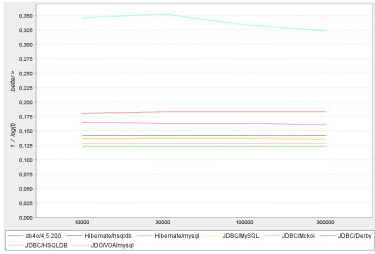
\includegraphics[height=4in]{/home/basedul/Documents/Report-writing-using-latex/ResturentManagementSystemReport/compari.png}
		\caption{Database comparison diagram \cite{Ref:6}}
		\label{fig:compari} 
	\end{figure}
\subsubsection{Normalisation}
Normalisation comes in many forms ranging from first normal form to sixth normal form. The nor-
malisation of a database is a systematic way to free the database of undesirable characteristics where
inserts, updates and deletions of data could lead to the loss of data integrity. The greater the normal
form, the greater the data integrity of the database.\\
The database in this system was designed to be in Boyce-Codd normal form which is a slightly
stronger version of the third normal form. For the database to be in Boyce-Codd normal form, it had
to pass for all previous normal forms as well as Boyce-Codd normal form.\\
A well designed database will normally abide by the first, second and third normal forms as they
are the basics to a well structured relational database. According to Horsforth School [17], the first
three normal forms can be defined as:
\begin{itemize}
	\item Every attribute is atomic or single valued therefore there are no repeating fields.
	\item All attributes not part of the primary key must be dependent on the full key.
	\item There must be no transitive determinants, or each attribute that is not part of
the key must be determined only by the key.
\end{itemize}
Finally for the database to be in the desired Boyce-Codd normal form, all tables must abide by the
first, second and third normal forms and must not have any determinants that are not candidate keys
for the table.
\subsubsection{Entity Relationship Diagram}
An entity relationship (ER) diagram is a modelling language used to represent a type of semantic
data model of a system. The ER diagrams are often used to represent a relational database and its
requirements in a top-down fashion usually defined as the database schema. The database schema for
this database has been split into two ER diagrams (Figures \ref{fig:entityone} and \ref{fig:entitytwo}).
Figure \ref{fig:entityone} graphically shows the objects and their relationships that are contained within a meal.
The meal object will be made of at least two ingredients that can be either a normal ingredient or
a prepared ingredient. Note, a prepared ingredient is a collection of ingredients used to either group
commonly used ingredients or to group optional ingredients. Each ingredient will have a default and
manual measurement with the default measurement entered on input of the ingredient and the manual
measurement entered if the meal ingredient link requires a different amount.
Also, each ingredient will be part of a generic ingredient object as there are many ingredients that
are the same item but packaged in a different way at a different price. This allows the database to be in
Boyce-Codd normalised state. An example of this would be the drink Coca-Cola which can be bought
by bottle, can or draught, thus are the same item but packaged differently at a different price and
amount. Finally each ingredient and prepared ingredient can be part of a category allowing optional
ingredients to be interchanged with other ingredients in the same category.
Figure \ref{fig:entitytwo} graphically shows the relationships for the menu, order and offer objects. The menu
consists of a date time relationship that provides the intervals to when the menu is active and a menu
section relationship that contains the colour variables and items under that particular menu section.
The order consists of one to many suborders with the suborder consisting of one to many items.
The order stores all the ingredients within each item and also the replaced ingredient if that optional
ingredient was replaced.
The offer consists of a date time relationship that provides the intervals to when the offer is active
and a offer section relationship that contains the sets required by the offer.
\begin{figure}[H]
		\centering
		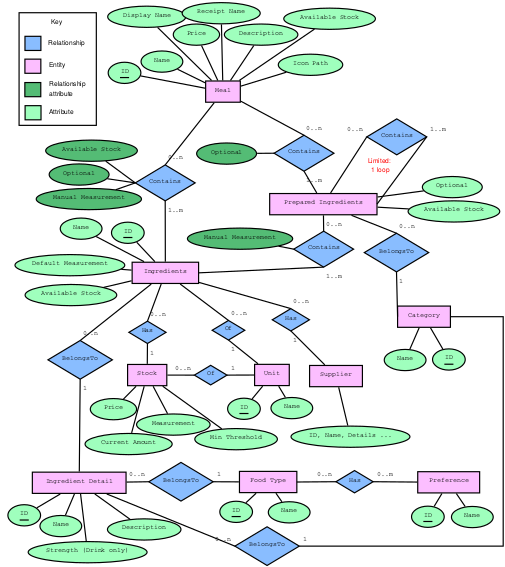
\includegraphics[height=6.5in]{/home/basedul/Documents/Report-writing-using-latex/ResturentManagementSystemReport/entityone.png}
		\caption{Entity Relationship diagram of a meal.}
		\label{fig:entityone} 
	\end{figure}
\begin{figure}[H]
		\centering
		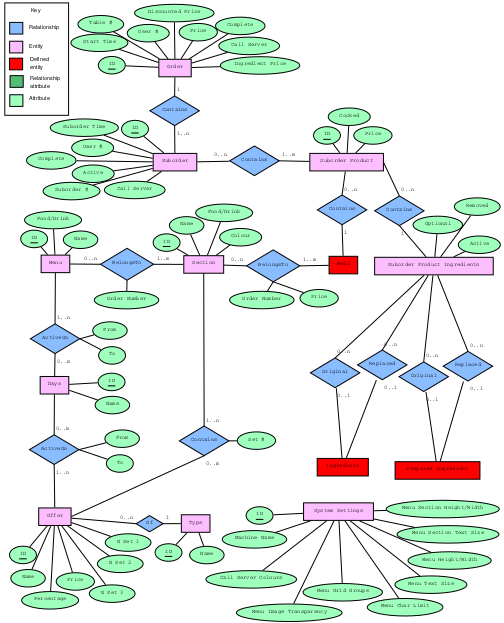
\includegraphics[height=6.5in]{/home/basedul/Documents/Report-writing-using-latex/ResturentManagementSystemReport/entitytwo.png}
		\caption{Entity Relationship of the menu, order and system settings.}
		\label{fig:entitytwo} 
	\end{figure}
\subsection{Flow Charts}
	A flow chart is a diagram used to represent the process flow of an algorithm, problem or some transaction
within a business. Therefore a flow chart (Figure \ref{fig:flowchart}) was used to graphically represent the process
flow of an order.
\begin{figure}[H]
		\centering
		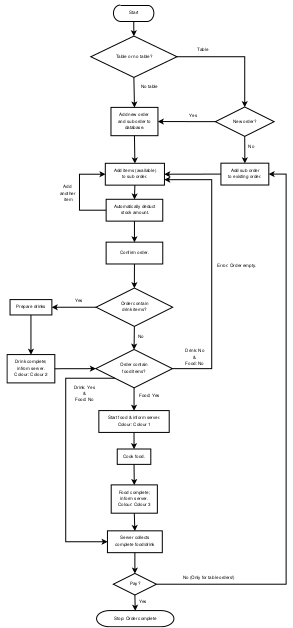
\includegraphics[height=6.5in]{/home/basedul/Documents/Report-writing-using-latex/ResturentManagementSystemReport/flowchart.png}
		\caption{Flow chart to show the flow of events of an order..}
		\label{fig:flowchart} 
\end{figure}
\subsection{Chapter Summary}
	This chapter has displayed many graphical representations of the design of the system. The imple-
mentation of the system is documented in the next chapter.
\newpage
\bibliographystyle{IEEEtran}
\bibliography{/home/basedul/Documents/Report-writing-using-latex/ResturentManagementSystemReport/req.bib}


\end{document}
